%%% The main file. It contains definitions of basic parameters and includes all other parts.

%% Settings for single-side (simplex) printing
% Margins: left 40mm, right 25mm, top and bottom 25mm
% (but beware, LaTeX adds 1in implicitly)
\documentclass[12pt,a4paper]{report}
\setlength\textwidth{145mm}
\setlength\textheight{247mm}
\setlength\oddsidemargin{15mm}
\setlength\evensidemargin{15mm}
\setlength\topmargin{0mm}
\setlength\headsep{0mm}
\setlength\headheight{0mm}
% \openright makes the following text appear on a right-hand page
\let\openright=\clearpage

%% Settings for two-sided (duplex) printing
% \documentclass[12pt,a4paper,twoside,openright]{report}
% \setlength\textwidth{145mm}
% \setlength\textheight{247mm}
% \setlength\oddsidemargin{14.2mm}
% \setlength\evensidemargin{0mm}
% \setlength\topmargin{0mm}
% \setlength\headsep{0mm}
% \setlength\headheight{0mm}
% \let\openright=\cleardoublepage

%% Generate PDF/A-2u
\usepackage[a-2u]{pdfx}

%% Character encoding: usually latin2, cp1250 or utf8:
\usepackage[utf8]{inputenc}

%% Prefer Latin Modern fonts
\usepackage{lmodern}

%% Further useful packages (included in most LaTeX distributions)
\usepackage{amsmath}        % extensions for typesetting of math
\usepackage{amsfonts}       % math fonts
\usepackage{amsthm}         % theorems, definitions, etc.
\usepackage{bbding}         % various symbols (squares, asterisks, scissors, ...)
\usepackage{bm}             % boldface symbols (\bm)
\usepackage{graphicx}       % embedding of pictures
\usepackage{fancyvrb}       % improved verbatim environment
\usepackage{natbib}         % citation style AUTHOR (YEAR), or AUTHOR [NUMBER]
\usepackage[nottoc]{tocbibind} % makes sure that bibliography and the lists
			    % of figures/tables are included in the table
			    % of contents
\usepackage{dcolumn}        % improved alignment of table columns
\usepackage{booktabs}       % improved horizontal lines in tables
\usepackage{paralist}       % improved enumerate and itemize
\usepackage{xcolor}         % typesetting in color

%% Path to images
\graphicspath{ {../img/} }

%%% Basic information on the thesis

% Thesis title in English (exactly as in the formal assignment)
\def\ThesisTitle{Automated Program Minimization With Preserving of Runtime Errors}

% Author of the thesis
\def\ThesisAuthor{Denis Leskovar}

% Year when the thesis is submitted
\def\YearSubmitted{2021}

% Name of the department or institute, where the work was officially assigned
% (according to the Organizational Structure of MFF UK in English,
% or a full name of a department outside MFF)
\def\Department{Department of Distributed and Dependable Systems}

% Is it a department (katedra), or an institute (ústav)?
\def\DeptType{Department}

% Thesis supervisor: name, surname and titles
\def\Supervisor{doc. RNDr. Pavel Parízek, Ph.D.}

% Supervisor's department (again according to Organizational structure of MFF)
\def\SupervisorsDepartment{Department of Distributed and Dependable Systems}

% Study programme and specialization
\def\StudyProgramme{Computer Science}
\def\StudyBranch{System Programming}

% An optional dedication: you can thank whomever you wish (your supervisor,
% consultant, a person who lent the software, etc.)
\def\Dedication{%
Dedication.
}

% Abstract (recommended length around 80-200 words; this is not a copy of your thesis assignment!)
\def\Abstract{%
Debugging~of large programs is a~difficult and time consuming task.
Given~a runtime error, the~developer must first reproduce it. 
He then has~to find the cause~of the~error and create a~bugfix.
This process can be made significantly more efficient by reducing 
the amount~of code the developer has~to look into. 
This paper introduces three different methodologies~of automatically reducing
a~given program $P$ into its minimal runnable subset $P'$.
The automatically generated program $P'$ also has~to result~in the~same runtime
error as~$P$.
The main focus~of the reduction is on~correctness when operating in a~concrete
application domain set by this study.
Implementations~of introduced methodologies written using the~LLVM compiler
infrastructure are then compared and classified.
Performance is measured based~on the statement count~of the~newly generated
program and the~speed at which the~minimal variant was generated.
Moreover, the~limits of the~three different approaches are investigated
with respect~to~the general application domain.
The~paper concludes with an~overview~of the~most general and efficient methodology.
}

% 3 to 5 keywords (recommended), each enclosed in curly braces
\def\Keywords{%
{automated debugging}, {code analysis}, {syntax tree}, {statement reduction}, {clang}
}

%% The hyperref package for clickable links in PDF and also for storing
%% metadata to PDF (including the table of contents).
%% Most settings are pre-set by the pdfx package.
\hypersetup{unicode}
\hypersetup{breaklinks=true}

% Definitions of macros (see description inside)
%%% This file contains definitions of various useful macros and environments %%%
%%% Please add more macros here instead of cluttering other files with them. %%%

%%% Minor tweaks of style

% These macros employ a little dirty trick to convince LaTeX to typeset
% chapter headings sanely, without lots of empty space above them.
% Feel free to ignore.
\makeatletter
\def\@makechapterhead#1{
  {\parindent \z@ \raggedright \normalfont
   \Huge\bfseries \thechapter. #1
   \par\nobreak
   \vskip 20\p@
}}
\def\@makeschapterhead#1{
  {\parindent \z@ \raggedright \normalfont
   \Huge\bfseries #1
   \par\nobreak
   \vskip 20\p@
}}
\makeatother

% This macro defines a chapter, which is not numbered, but is included
% in the table of contents.
\def\chapwithtoc#1{
\chapter*{#1}
\addcontentsline{toc}{chapter}{#1}
}

% Draw black "slugs" whenever a line overflows, so that we can spot it easily.
\overfullrule=1mm

%%% Macros for definitions, theorems, claims, examples, ... (requires amsthm package)

\theoremstyle{plain}
\newtheorem{thm}{Theorem}
\newtheorem{lemma}[thm]{Lemma}
\newtheorem{claim}[thm]{Claim}

\theoremstyle{plain}
\newtheorem{defn}{Definition}

\theoremstyle{remark}
\newtheorem*{cor}{Corollary}
\newtheorem*{rem}{Remark}
\newtheorem*{example}{Example}

%%% An environment for proofs

\newenvironment{myproof}{
  \par\medskip\noindent
  \textit{Proof}.
}{
\newline
\rightline{$\qedsymbol$}
}

%%% An environment for typesetting of program code and input/output
%%% of programs. (Requires the fancyvrb package -- fancy verbatim.)

\DefineVerbatimEnvironment{code}{Verbatim}{fontsize=\small, frame=single}

%%% The field of all real and natural numbers
\newcommand{\R}{\mathbb{R}}
\newcommand{\N}{\mathbb{N}}

%%% Useful operators for statistics and probability
\DeclareMathOperator{\pr}{\textsf{P}}
\DeclareMathOperator{\E}{\textsf{E}\,}
\DeclareMathOperator{\var}{\textrm{var}}
\DeclareMathOperator{\sd}{\textrm{sd}}

%%% Transposition of a vector/matrix
\newcommand{\T}[1]{#1^\top}

%%% Various math goodies
\newcommand{\goto}{\rightarrow}
\newcommand{\gotop}{\stackrel{P}{\longrightarrow}}
\newcommand{\maon}[1]{o(n^{#1})}
\newcommand{\abs}[1]{\left|{#1}\right|}
\newcommand{\dint}{\int_0^\tau\!\!\int_0^\tau}
\newcommand{\isqr}[1]{\frac{1}{\sqrt{#1}}}

%%% Various table goodies
\newcommand{\pulrad}[1]{\raisebox{1.5ex}[0pt]{#1}}
\newcommand{\mc}[1]{\multicolumn{1}{c}{#1}}

%%% Coding packages for pseudocode
\usepackage{algorithm} 
\usepackage{algpseudocode} 
\usepackage{listings}
\lstset
{
	frame=tlrb,
	numbers=left,
	breaklines=true,
	breakatwhitespace=true,
}

%%% Todo notes
\usepackage{xargs}	% Use more than one optional parameter in a new commands
\usepackage[colorinlistoftodos,prependcaption,textsize=tiny]{todonotes}
\newcommandx{\unsure}[2][1=]{\todo[linecolor=red,backgroundcolor=red!25,bordercolor=red,#1]{#2}}
\newcommandx{\change}[2][1=]{\todo[linecolor=blue,backgroundcolor=blue!25,bordercolor=blue,#1]{#2}}
\newcommandx{\info}[2][1=]{\todo[linecolor=OliveGreen,backgroundcolor=OliveGreen!25,bordercolor=OliveGreen,#1]{#2}}
\newcommandx{\improvement}[2][1=]{\todo[linecolor=Plum,backgroundcolor=Plum!25,bordercolor=Plum,#1]{#2}}
\newcommandx{\thiswillnotshow}[2][1=]{\todo[disable,#1]{#2}}

% Title page and various mandatory informational pages
\begin{document}
%%% Title page of the thesis and other mandatory pages

%%% Title page of the thesis

\pagestyle{empty}
\hypersetup{pageanchor=false}
\begin{center}

\centerline{\mbox{
\includegraphics[width=166mm]{../img/logo-en.pdf}}}

\vspace{-8mm}
\vfill

{\bf\Large BACHELOR THESIS}

\vfill

{\LARGE\ThesisAuthor}

\vspace{15mm}

{\LARGE\bfseries\ThesisTitle}

\vfill

\Department

\vfill

{
\centerline{\vbox{\halign{\hbox to 0.45\hsize{\hfil #}&\hskip 0.5em\parbox[t]{0.45\hsize}{\raggedright #}\cr
Supervisor of the bachelor thesis:&\Supervisor \cr
\noalign{\vspace{2mm}}
Study programme:&\StudyProgramme \cr
\noalign{\vspace{2mm}}
Study branch:&\StudyBranch \cr
}}}}

\vfill

% Zde doplňte rok
Prague \YearSubmitted

\end{center}

\newpage

%%% Here should be a bound sheet included -- a signed copy of the "bachelor
%%% thesis assignment". This assignment is NOT a part of the electronic
%%% version of the thesis. DO NOT SCAN.

%%% A page with a solemn declaration to the bachelor thesis

\openright
\hypersetup{pageanchor=true}
\pagestyle{plain}
\pagenumbering{roman}
\vglue 0pt plus 1fill

\noindent
I declare that I carried out this bachelor thesis independently, and only with the cited
sources, literature and other professional sources. It has not been used to obtain another
or the same degree.

\medskip\noindent
I understand that my work relates to the rights and obligations under the Act No.~121/2000 Sb.,
the Copyright Act, as amended, in particular the fact that the Charles
University has the right to conclude a license agreement on the use of this
work as a school work pursuant to Section 60 subsection 1 of the Copyright~Act.

\vspace{10mm}

\hbox{\hbox to 0.5\hsize{%
In \hbox to 6em{\dotfill} date \hbox to 6em{\dotfill}
\hss}\hbox to 0.5\hsize{\dotfill\quad}}
\smallskip
\hbox{\hbox to 0.5\hsize{}\hbox to 0.5\hsize{\hfil Author's signature\hfil}}

\vspace{20mm}
\newpage

%%% Dedication

\openright

\noindent
\Dedication

\newpage

%%% Mandatory information page of the thesis

\openright

\vbox to 0.5\vsize{
\setlength\parindent{0mm}
\setlength\parskip{5mm}

Title:
\ThesisTitle

Author:
\ThesisAuthor

\DeptType:
\Department

Supervisor:
\Supervisor, \SupervisorsDepartment

Abstract:
\Abstract

Keywords:
\Keywords

\vss}

\newpage

\openright
\pagestyle{plain}
\pagenumbering{arabic}
\setcounter{page}{1}


%%% A page with automatically generated table of contents of the bachelor thesis

\tableofcontents

%%% Each chapter is kept in a separate file
\chapter*{Introduction}
\addcontentsline{toc}{chapter}{Introduction}

\change[inline]{TODO: Rewrite the~introduction to include goals.}

Automation of~routine tasks tied with software development has resulted in a~tremendous
increase in the~productivity of~software engineers. 

However, the~task of~debugging a~program
remains mostly manual chore. 
This is due to the~difficulty of~reliably encountering logic-based
runtime errors in the~code, a~task that, to this day, requires 
the developer's attention and supervision.

Let program $\mathcal{P}$ contain a~runtime error $E$ 
that consistently occurs when $\mathcal{P}$ is run 
with arguments $A$.
Since the~error $E$ is present at runtime and not compile-time,
it can be assumed that syntax wise the~code is mostly correct.
Therefore, any syntax-based error can be ruled out.
This, in turn, leaves us with a~set of~logical errors $\mathcal{E_L}$.
Those include wrongly indexed arrays and calculations that lead to either
the incorrect result or an altered control flow of~the program. 
Let $E \in \mathcal{E_L}$. As the~generality of~errors in $\mathcal{E_L}$
appears too complicated to be solved for all programming languages at once, 
it is necessary to break the~problem down for each programming language. 
This article is concerned with the~logical errors of~C and C++.
Although C is not a~subset of~C++, the~logical errors made in C can be
approached similarly to those in C++.
Both languages share mostly comparable constructs.
Finding the~cause of~a logical error in a~concrete language requires knowing
these constructs, their behavior, and their general handling.

To make finding the~cause of~an error a~systematic approach, one might try removing
unnecessary statements in the~code, thus minimizing the~program.
Let $\mathcal{P'}$ be a~minimal variant of~$\mathcal{P}$ such 
that $\mathcal{P'}$ results in the~same error $E$ as $\mathcal{P}$
when run with the~same arguments $A$.
If done carefully and correctly, $\mathcal{P'}$ represents the~smallest 
subset of~$\mathcal{P}$ regarding code
size, while preserving the~cause of~the error in that subset.
Upon manual inspection, the~developer is required to make less of~an effort to find
the cause in $\mathcal{P'}$ as opposed to $\mathcal{P}$.

The minimization of~a program can be achieved in numerous ways.
In further sections, the~article describes and compares three different approaches.
The first is based on naive statement removal and its consequences during runtime.
The second removes major chunks of~the code while
periodically testing the~generated program's correctness.
The third deploys a~sequence of~code
altering techniques, namely slicing and delta debugging.


\chapter{Automated debugging techniques}

\change[inline]{TODO: Link relevant literature from Slicing of LLVM bitcode (muni.cz) and Bobox Runtime Optimization (cuni.cz)}

Debugging can be described as the process of analyzing erroneous code to find 
the cause of those errors.
While most developers see debugging as a manual chore, there were numerous 
attempts~ at automating at least some parts of it during the last few decades. 
The rise in popularity of program analysis resulted in automated error checks 
for popular programming languages. 

While these checks mostly cover only specific 
cases~of potential bugs, such as out-of-range array indexing, they have proven 
themselves as a useful tool for the developer. In the context of this work, 
such checks provide a helping hand at a low cost when minimizing a program. 

The following sub-chapters will talk about the techniques behind such checks 
and how they deal with automated debugging.

\section{Delta debugging}

Delta debugging is an iterative approach described by Zeller in 1999. 
It does not perform any static analysis of the debugged program, as it 
is~not meant to find failures in the code. 

Delta debugging instead intends to 
minimize the debugged program's incorrect input to isolate the input's 
failure-inducing part. 
Therefore, it requires the program in question and the specific input 
and the expected output. 
In other words, Delta debugging requires a set of test cases, which attempts to 
minimize and isolate the failure-inducing input. Minimality is defined as follows.

\begin{defn}[Test case]\label{def02:1}
  Let $c_\mathcal{F}$ be a set of all changes $\delta_1,\dots,\delta_n$ 
  between a passing program run $r_\mathcal{P}$ and a failing program run
  $r_\mathcal{F}$ such that 
  \begin{align}
	r_\mathcal{F} = (\delta_1(\delta_2(\dots(\delta_n(r_\mathcal{P}))))). \nonumber 
  \end{align}
  We call a subset $c \subseteq c_\mathcal{F}$ a \emph{test case}.
\end{defn}

\begin{defn}[Global minimum]\label{def02:2}
  A test case $c \subset c_\mathcal{F}$ is called a \emph{global minimum}
  of $c_\mathcal{F}$ if $\forall c_i \subseteq c_\mathcal{F}:
  (|c_i| < |c| \implies c_i$ does not cause the program to fail.$)$
\end{defn}

Global minimum can be interpreted as the smallest set of changes able to
make the program fail.

\begin{defn}[Local minimum]\label{def02:3}
  A test case $c \subset c_\mathcal{F}$ is called a \emph{local minimum}
  of $c_\mathcal{F}$ if $\forall c_i \subseteq c:
  (c_i$ does not cause the program to fail.$)$
\end{defn}

\begin{defn}[$n$-minimality]\label{def02:4}
  A test case $c \subset c_\mathcal{F}$ is \emph{$n$-minimal}
  if $\forall c_i \subseteq c:
  (|c| - |c_i| \leq n \implies c_i$ does not cause the program to fail.$)$
\end{defn}

The minimizing Delta debugging algorithm attempts to find a 1-minimal test case.

Delta debugging seems to bet on the premise that large-scale applications are written
with automated testing in mind. On the same note, it is the recommended practice to
develop programs while at the same time dedicating resources to write tests for that
program.

The defined minimality can be used to construct the minimizing algorithm. 
However, the delta debugging algorithm can be easily and more comprehensively explained 
without the definition as well.

\begin{algorithm}
	\caption{Minimizing Delta Debugging Algorithm} 
	\begin{algorithmic}[1]
		\State $n \leftarrow 2$
		\State Split a string $S$ into $\alpha_1,\dots,\alpha_n$ of equal size.
		\State For each $\alpha_i$, calculate its complement $\beta_i$.
		\State Run tests on $\alpha_1,\dots,\alpha_n,\beta_1,\dots,\beta_n$.
		\If{all tests passed}
			\State $n \leftarrow 2*n$
			\If{$n > |\sigma|$}
				\Return the most recent failure causing substring.
			\Else
				\State goto (2).
			\EndIf
		\ElsIf{$\alpha_i failed$}
			\State $n \leftarrow 2$.
			\State $\sigma \leftarrow \alpha_i$.
			\If{$|\sigma| == 1$}
				\Return $\sigma$.
			\Else
				\State goto (2).
			\EndIf
		\Else
			\Comment $\beta_i$ failed.
			\State $\sigma \leftarrow \beta_i$.
			\State $n \leftarrow n - 1$.
			\State goto (2).
		\EndIf
	\end{algorithmic} 
\end{algorithm}

Additionally, minimizing is not the only approach Delta debugging suggests.
A more sophisticated one is isolation. Minimization can be described as removing parts
while the failure persists, which means that the output changes are only made in failing
iterations.
Isolation extends this by adding failure-inducing differences while the program passes tests.
This addition results in changes in both the passing and failing iterations.

One can quickly transform the input minimalization of Delta debugging into either source
code minimalization or error isolation at both the compile-time and runtime.
This transformation can be achieved for the compile-time by first setting the input
as the debugged program's source code. 
Second, it is required to set the expected
output to either 'compiled' or 'failed to compile'. 
Finally, the input is fed into a compiler, for example, GCC, which produces
one of the two set outputs. 

The runtime variant only differs in two points—first, changing the expected outputs. 
Second, changing the compiler to a compiler-debugger pipeline so that the source 
can be compiled and run.

\section{Static slicing}

The first introduced slicing method was static backward slicing. 
In 1984, Weiser defined a slice with respect to criterion C 
as a part of a program that potentially affects given variables in a given point. 

\begin{defn}[Static slicing criterion]\label{def02:5}
  Let $\mathcal{P}$ be a program consisting of program points 
  $P = p_1,\dots,p_n$ and variables $V = v_1,\dots,v_m$.
  Any pair $C = (p_i, V')$, such that $p_i \in P$, $V' \subseteq V$, and 
  $\forall v_i \in V': v_i$ is present in $p_i$, 
  is called a \emph{slicing criterion}.
\end{defn}

Slicing is the process of finding such a part of a program. 
Suggested approaches neglected any execution information and 
focused solely on observations made by analyzing the code.

\change[inline]{TODO: Convert the pseudocode to an easily readable
version (i.e. comparison with the non-sliced program).}

\begin{algorithm}
	\caption{Simple Branching Program} 
	\begin{algorithmic}[1]
		\State $x \leftarrow 1$
		\State $a \leftarrow$ read($a$)
		\For{$i = 1,2,\dots,C$}
			\State write($i$)
		\EndFor
		\If{$a$ mod $2 == 0$}
			\If{$a \neq 0$}
				\State $x \leftarrow -1 * x$
			\Else
				\State $x \leftarrow 0$
			\EndIf
		\Else
			\State $x \leftarrow x + 1$.
		\EndIf
		\State write($x$)
	\end{algorithmic}
\end{algorithm}

\begin{algorithm}
	\caption{Static Slice of the Simple Branching Program} 
	\begin{algorithmic}[1]
		\State $x \leftarrow 1$
		\State $a \leftarrow$ read($a$)
		\If{$a$ mod $2 == 0$}
			\If{$a \neq 0$}
				\State $x \leftarrow -1 * x$
			\Else
				\State $x \leftarrow 0$
			\EndIf
		\Else
			\State $x \leftarrow x + 1$.
		\EndIf
		\State write($x$)
	\end{algorithmic}
\end{algorithm}

Later that year, Ottenstein and Ottenstein restated the problem as a reachability
search in the program dependence graph (PDG).
PDG represents statements in the code as vertices and data and control
dependencies as oriented edges. 
Additionally, edges induce a partial ordering on the vertices. 
In order to preserve the semantics of the program, statements must be executed 
according to this ordering. 

Edges are, therefore, of two types. 
First, the control dependency edge specifies that an incoming vertex's 
execution depends on the outgoing one's execution. 
Second, the data flow dependence edge suggests that a variable appearing
in both the outgoing and incoming edge share a variable,
the value of which depends on the order of the vertices execution.

Once the PDG is built, slices can be extracted in linear time 
with respect to the number of vertices.

\change[inline]{TODO: Show how PDG is sliced, from 2.2 Slicing of LLVM bitcode (muni.cz)}

However, one can find many potential issues and obstacles when performing 
data flow analysis. 
Omitting the interprocedural slicing, as it is not relevant in this paper's
context, one is left with pointers and unstructured control flow.
While the latter is seldomly used in single-threaded modern programming, 
the same cannot be said about the former. 

Pointers require us to extend the syntactic data flow analysis 
into a pointer or points-to analysis, which should be performed first. 
It is necessary to keep track of where pointers may point to (or must point to,
in case their address is not reassigned) during the execution. 
From this knowledge, other data flow edges must be created or
changed to accommodate the fact when the outgoing vertex mayhap writes
into a memory location possibly used by the incoming vertex. 

The analogical approach is then used for control dependency analysis since 
pointers might alter control flow as well. 
This change to control flow happens, namely when functions are called using 
function pointers.

The main advantage of static slicing is that it does not require
any runtime information. 
As program execution can be expensive both time-wise and resource-wise, 
static slicing offers program comprehension at a low cost. 
Because static slicing discovers program statements that can affect 
certain variables, it can remove dead code and be used for program segmentation. 

Furthermore, static slicing is used for testing software quality, maintenance, 
and test, all of which are relevant to this project.

\section{Dynamic slicing}

While the idea of building a program slice prevails, dynamic slicing 
drastically differs from static slicing in terms of input and the way
it is processed. 

In 1988, Korel and Laski described a slicing approach that took into 
consideration information regarding a program's concrete execution. 
As opposed to static slicing, which builds a slice for any execution, 
dynamic slicing builds a slice for a given execution of a program. 
Using information available during a run of the program 
results in a typically much smaller slice.

\change[inline]{TODO: Convert the pseudocode to an easily readable
version (i.e. comparison with the non-sliced program).}

\begin{algorithm}
	\caption{Dynamic Slice of the Simple Branching Program (for $a = 2$)} 
	\begin{algorithmic}[1]
		\State $x \leftarrow 1$
		\State $a \leftarrow$ read($a$)
		\State $x \leftarrow 0$
		\State write($x$)
	\end{algorithmic}
\end{algorithm}

This decrease in size is mainly due to removing unnecessary 
branching of control statements and unexecuted statements in general. 
The slicing criterion now contains a set of the program's 
arguments in addition to the previous information. 
The location of the criterion's statement is also specified to avoid 
vagueness in the execution history. 

The criterion is therefore defined as follows.

\begin{defn}[Dynamic slicing criterion]\label{def02:5}
  Let $\mathcal{H} = (s_{x1},\dots,s_{xn})$ be an execution history of a program 
  $\mathcal{P} = (\{s_1,\dots,s_m\}, V)$, where $s_i$ denotes a statement
  and V is a set of variables $v_1,\dots,v_k$.
  Any triple $C = (h_i, V', \{a_1,\dots,a_j\})$, such that $h_i \in \mathcal{H}$,
  $V' \subseteq V$, $\forall v_i \in V': v_i$ is present in $h_i$,
  and $\{a_1,\dots,a_j\}$ is the input of the program,
  is called a \emph{slicing criterion}.
\end{defn}

Since dynamic slicing requires the user to run the program, 
it is typically used in cases where the execution with a fixed 
input happens regardless. Such cases include debugging and testing. 
For debugging, dynamic slices must reflect the subsequent restriction: 
a program and its slices must follow the same execution paths.

\section{Summary}

While the described program minimizing and debugging approaches have been 
formulated more than two decades ago, there have not been nearly enough 
successful attempts at implementing them. 

With each approach having its clear positives and negatives, 
it would be interesting to see how they handle program minimization. 
When cleverly used, a combination of these methods might 
result in a reasonably fast and inexpensive algorithm 
for the reduction of program size.
\chapter{Compilers and analysis tools}

In the~previous chapter, the~reader was introduced to a~branch of~program
ana\-ly\-sis. 
The techniques discussed above focused on both the~static and runtime
side of~program analysis. 

Regardless of~whether these approaches have been implemented, it was 
required to find a~suitable tool for source code manipulation for two reasons. 
First, any external tool output might require altering the~input source code 
based on its output. 
Second, if implementing any code reducing algorithm would have to occur, 
one would need a~sophisticated code modifying framework. 

Due to these reasons, an analysis of~compilers and tools for C and C++ was conducted. 
The goal of~the~analysis is to pick the~most practical tool available. 
Required criteria include frequent upkeep of~the~framework, 
an existing user base, and the~ability to manipulate some abstract 
representation of~the~code.

The representation boiled down to an abstract syntax tree (AST). 
AST embodies the~syntactic structure of~the~code, regardless of~the~code's language. 
A vertex of~an AST represents a~construct of~the~code while not being concrete 
with the~details of the code's programming language. 
This generality is perfect for C and C++'s chosen domain, 
as both languages only differ syntax-wise in~minor details.

Below are the~findings concerning the~most important candidates.

\section{GCC}

A well-known C and C++ compiler, the~GNU Compiler Collection \citep{gcc:online} 
is an extensive
open source project. 
As popular as GCC is, it does not provide the~features an analysis-tool-building 
developer needs. 

For the~sake of~building such tools, a~compiler front end is used. 
Due to an old design, it is difficult to work with either the~front end or 
the back end of~GCC alone. 
Besides, the~compiler implicitly makes optimizations that destroy any parallels 
between the~source code and the~AST. 
Therefore, the~AST has to be treated as an entirely different object rather than 
an abstraction of~the~code. 
Most of~the~compiler's source code representation is unintuitive and 
hard to pick up for anyone not actively contributing to GCC. 
Figure~\ref{img:gcc} showcases the~unfriendliness rather well.
Compared to figure~\ref{img:pdg}, which is an output of~a~tool built using
LLVM and Clang, GCC's mapping between the~source code and the~internal
representation does not hold up.

As far as AST manipulation is concerned, the~compiler allows the~user to dump 
the structure into a~text representation. 
However, due to the~difficulties mentioned above, it can hardly be used.

\begin{figure}[p]\centering
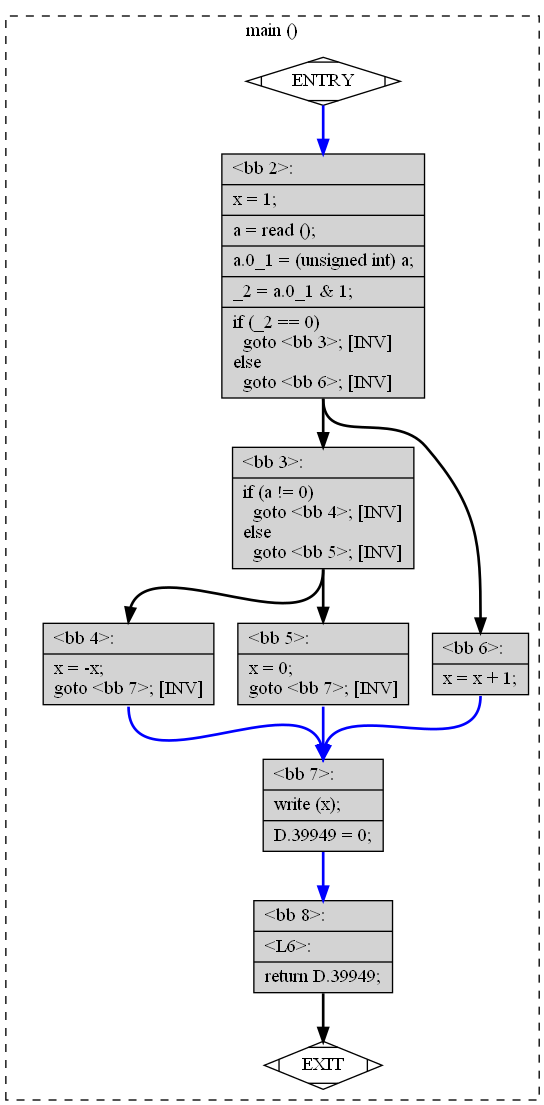
\includegraphics[scale=0.55]{gcc_ast}
\caption{GCC AST Dump. This figure showcases 
the AST representation of~\ref{lst:simpleexample}
as dumped by GCC. Note that it is not easily comprehendable.}
\label{img:gcc}
\end{figure}

These issues result in~a seldom-used variant that offers nearly 
no developer-friendly features. 
An upside is that GCC allows the~user to visualize the~AST. 
However, that is hardly a~useful feature in~the context of~this paper.

\section{Clang}

Thanks to LLVM \citep{llvm:online}, the~widespread compiler infrastructure,
the Clang project \citep{clang:online}
has provided a~compiler front end not only for C and C++ but also 
for CUDA, OpenCL, and other mainstream programming languages. 
The extend of~Clang as a~compiler front end is so vast that it covers 
both the~C++ standard and the~unofficial GNU++ dialect.

The project does not include just the~front end but also a~static analyzer 
and several code analysis tools, which are now commonly used in~IDE's as 
syntax and semantic checks. 

This description of~Clang foreshadows its friendliness to analysis tool developers. 
The fact that the~front end runs on a~common intermediate language also indicates 
that openly working with abstract code representations is supported.

There are three most notable interfaces for customizing Clang. 
Firstly, the LibClang interface allows the~users to write 
comprehend-able high-level code with limited functionality. 
On the~other hand, LibTooling gives the~user much more control 
at the~cost of~a~steep learning curve. 
Lastly, the~Plugins interface features similar difficulty 
as LibTooling with a~more specific goal. 
Plugins are used with the~Clang compiler and can be run 
as a~front-end action when called during compilation.

\section{ANTLR}

A less typical way of~extracting an AST from a~source file is by using grammar
recognition.
ANTLR \citep{antlr:online}, which stands for Another Tool for 
Language Recognition, is a~free 
parser generator that generates both a~lexer and a~parser based on 
a given grammar.
Additionally, ANTLR can also generate a~tree parser.
Tree parsers are helpful in~processing ASTs.

The tool is generally used to read data formats, process expressions 
of various query languages, and even parse source code written in complex 
programming languages.
It can be used to generate a~syntax tree and walk through it using a~visitor.
ANTLR is based on the~LL parser, which parses the~input from left to right, 
performing its leftmost derivation.

To create a~parser or a~syntax tree of~code written in a~programming language, 
ANTLR requires the complete grammar of~that language.
Some programming languages, namely C and C++, have an ambiguous syntax that 
is hard to parse based solely on its grammar.
Due to ANTLR's high popularity, many grammars have already been written 
for it.
As far as C++ is concerned, its C++14 standard's grammar is the~most recent 
one available.

Writing grammar for newer standards or creating a~custom one for both C and 
C++ would be unnecessarily burdensome for this project.
This statement holds, especially when considering other tools mentioned above.

The most recent release, ANTLR 4, added more options for grammar rules.
Most notably, it supports direct left recursion.
However, that still might not be enough to choose it over other tools.


\section{DMS}

Similar to ANTLR, the~DMS Software Reengineering Toolkit \citep{dms:online}
features a~parser generator.
The tool is proprietary software created by Semantic Designs.
Besides the~mentioned parser generator, it features an entire toolkit for 
creating custom software analysis.
This toolkit is used mainly for reliable refactoring, duplicate code 
detection, and migration of the source code's programming language.

The parser generator part takes a~grammar and produces a~parser.
This parser then constructs abstract syntax trees for provided source code.
Additionally, created ASTs can be converted back to source code using 
prettyprinters.
The parser saves additional information about provided source files, such as 
comments and formatting.
It can then recreate the~file accurately.

DMS provides a~grammar for a~large number of~programming languages, 
including C and C++.
The language support, however, is not always up-to-date.
The newest supported C++ standard is still the~older C++17.
These complicated grammars' ambiguity is avoided using a~generalized 
left-to-right parser, which performs the~rightmost derivation (GLR).
Since DMS provides refactoring ability as well, it allows for transformation 
rules in~the grammar.

Another helpful feature of~the~toolkit is control flow and data flow analysis.
Analyzing control flow and data flow, generating their graphs, and performing 
the points-to analysis (also supported by DMS) is practical when considering
static slicing (section 1.2).

It should be noted that some of~the~free, open-source tools mentioned above 
do a~better job of~being a~so-called 'software analysis toolkit' than 
DMS does.

\section{Summary}

The chapter highlighted a~spectrum of~tools, ranging from language
recognizers to compilers.

It would seem that parsing source code written in multiple programming 
languages into an abstract representation requires a~common intermediate 
language, in~which the representation is stored. 
Having an intermediate language is not always possible for several reasons, 
including licensing and old architecture. 
The compiler giant GCC seems to suffer from precisely that.
Additionally, since the~Clang project is being contributed to regularly, 
resulting in~as many as five releases per year, 
it pulls in~a more significant developer community. 

Therefore, Clang is the~favorite source code altering tool for this project. 
In the~following chapter, the~relevant parts of~the~Clang project 
will be broken down and explained.

\chapter{Clang LibTooling}\label{chap:libtooling}

The previous chapter described tools and environments that were taken
into consideration for this project. 
The utmost importance was given to the~ease of~use, availability, and 
active community. 
As the~reader might have guessed from the~summary, the~LLVM/Clang 
suite stood out as the~best candidate.

Clang is a~language front-end. With high compilation performance, 
low memory footprint, and modifiable code base, it quickly and flexibly 
converts source code to LLVM intermediate code representation. 
The front-end supports languages and frameworks such as C/C++, 
Objective C/C++, CUDA, OpenCL, OpenMP, RenderScript, and HIP. 
This support is crucial for this thesis since the~project 
aims to support both C and C++. 
The LLVM Core then handles the~optimization and IR synthesis, 
supporting a~plethora of~popular CPUs.

Clang is widely used for its warnings and error checks, both very 
helpful and outstanding compared to competing compilers. 
Furthermore, Clang offers an extensive tooling infrastructure 
through which tools such as clang-tidy were developed. 
A relatively well-documented tooling API written in~C++ helps 
programmers create their tools easily. 
However, not all developers share the~same skill set. 
Some programmers require complicated additional features, while others 
prefer an easy-to-use interface. 
The tooling API has been split into multiple libraries and frameworks,
including Plugins and LibClang.
Explaining the two mentioned libraries is necessary. 
It is essential to show their capabilities before introducing LibTooling. 
LibTooling is the tooling library ultimately chosen for this project.

\paragraph{Plugins.}

The~library intuitively called Plugins is used for plugin development.
The library is linked dynamically, resulting in~relatively small tools.
Plugins are launched at compilation and offer compilation control as well 
as access to the~AST.

More specifically, Plugins allow performing an extra custom front-end action 
during compilation.
The functionality is generally similar to that of~LibTooling, which will be 
talked about later.
However, unlike a~standalone tool, Plugins cannot do any tasks before and after 
the analysis (and compilation).
When creating a~plugin, one can choose from a~selection of~
\icode{FrontendAction} classes to inherit.
If, for example, the~plugin should work with the~AST, 
the \icode{ASTFrontendAction} can be inherited.
Doing so also allows overriding the~\icode{ParseArgs} method, in~which 
the plugin's command line handling is specified.

Due to dynamic loading, the~wanted plugin must be added to a~plugin registry 
inside the~code.
The plugin is then loaded from the~registry by specifying the~\icode{-load} 
command or \icode{-fplugin} on the~command line when running clang.
The plugin takes those arguments from the~command line that are prefixed 
by \icode{-Xclang}.

\paragraph{LibClang.}

Another framework, LibClang, offers a~simple C and Python API for quick 
tool writing. 
Unlike Plugins and LibTooling, which will be mentioned later, the~code 
base of~LibClang is stable. 
This stability implies that tools written using LibClang do not require
upkeep with every new LLVM/Clang release. 
Overall, the~framework and tools written using it are high-level and 
are easily readable.

\paragraph{LibTooling.}

The most feature woven set of~libraries is LibTooling. 
Unlike Plugins, LibTooling \citep{libtooling:online} 
allows the~developer to build standalone 
Clang tools. 
This robust framework is written in~C++ and has an active 
community of~contributors. 
One can find many manuals and tutorials online. 
However, with each contribution to LibTooling and each release of~Clang, 
there is a~chance that older tools will not support the~newer LibTooling 
API. 
That is the~reason why countless tools written using this framework do not
run in~modern environments. 
Programmers who use LibTooling cannot expect compatibility in~upcoming 
releases. 
On the~bright side, the~libraries of~LibTooling allow a~plethora of~source
code modifications, AST traversals, and access to the~compiler's internals.

The set of~features supplied by LibTooling is immense. 
The following sections describe notable features used during 
the implementation of~this project. 
The reader should get a~better idea of~how a~tool is built and what 
LibTooling offers during the~development process. 
Important concepts, such as providing the~correct input to the~tool 
in the~form of~a~compilation database, traversing the~AST, 
and modifying source code inside the~tooling environment, 
are described below. 
These concepts will be referenced further in~the text.

\section{Compilation databases}

To accurately and faithfully recreate a~compilation, tools created using 
LibTooling require a~compilation database (CD) \citep{cd:online} 
for a~given input project.

The motivation behind a~CD is simple.
If a~source file uses unusual include paths that need to be provided 
using the~\icode{-I} compiler command, it cannot be reliably compiled.
Similarly, if the~file contains macros and lacks definitions, its content 
can drastically change when the~definitions are present.
In the~latter case, definitions are provided to the~compiler 
with the~\icode{-D} command.
Such compiler commands, options, and flags are usually defined in~a build 
system.
At least, that is the~recommended practice for larger projects.
Having a~build system is similar to having a~CD.
It is clear which file is compiled with which options.

Clang expects a~CD in~the JSON format and looks for the~file specifically
named  \icode{compile\_commands.json} in~the current or parent 
directories.
The JSON file contains entries for source files.
Each entry contains a~directory, a~file name, and a~compilation command.
Multiple entries for a~single source file are also valid.
Such a~case can arise when performing repeated compilation.

As previously mentioned, having a~build system helps.
Build tools such as CMake and Ninja can be used to generate a~CD.
If the~project is not using any of~the~compatible build tools, 
the user can either make a~CD manually or use an external tool.
One such tool is Build EAR available at \url{https://github.com/rizsotto/Bear}.

Tools created using LibTooling do not always require compilation databases 
to run.
For simple projects, they can take the~\icode{-{}-} argument that separates 
the tool's arguments from the~project's compilation arguments.
One can interpret the~arguments following \icode{-{}-} as a~temporary
compilation database.

\section{Clang AST}\label{chap:ast}

The abstract syntax tree used in~the Clang front-end \citep{ast:online}
is different from the~typical AST. 
It saves and carries more data, namely context.  
For example, it contains additional information to map source 
code to nodes and capture semantics. 
This chapter describes the Clang node type hierarchy, the tree's 
representation in memory, and different ways of traversing an AST.
\subsection{Node types}

Clang AST's nodes belong to a~vast class hierarchy. 
This hierarchy contains classes that represent every supported 
source code construct.
Nodes are of~four different types: statements (\icode{Stmt}), 
declarations (\icode{Decl}), specific declaration context 
(\icode{DeclContext}), and types (\icode{Type}). 
However, in~the APIs mentioned above, the~nodes do not share
a common ancestor.

The children of~\icode{Type} represent all available types.
The goal is to give each type in~the source code a~canonical type,
i.e., a~type stripped of~any typedef names. 
Canonical types are used for type comparison, while non-canonical 
types give complete information during diagnostics. 
The \icode{Decl} hierarchy's goal is to have a~class for each 
type of~declaration or definition. 
These declarations vary, and the~children cover specific cases 
such as function, structure, and enum declarations. 
Some declarations, such as function and namespace declarations, 
capture additional data in~\icode{DeclContext}'s children. 
The final node type, \icode{Stmt}, represents a~single statement. 
It has subclasses for loops, control statements, compound statements, 
and more. 
Additionally, expressions (\icode{Expr}) also belong 
to the~\icode{Stmt} hierarchy.

Figure~\ref{dia:ast} shows a~part of~the~class hierarchy. 
The entire class diagram cannot be shown as there are over a~thousand 
different classes\footnote{The class hierarchy is shown in~Clang's
Doxygen documentation. An example of~the~Stmt hierarchy can be found
at \url{https://clang.llvm.org/doxygen/classclang_1_1Stmt.html}.}. 
The topmost node, the~root, of~a~concrete Clang AST is called the~translation
unit declaration (\icode{TranslationUnitDecl}). 
Edges between nodes are simplified, as each node stores 
a container of~its children.

\begin{figure}[ht]\centering
\begin{tikzpicture}
	\begin{class}[text width=2cm]{Stmt}{-5.5, 0}
	\end{class}

	\begin{class}[text width=2.5cm]{ValueStmt}{-5.5, -6}		
		\inherit{Stmt}
	\end{class}

	\begin{class}[text width=2cm]{Expr}{-5.5, -8}
		\inherit{ValueStmt}
	\end{class}

	\begin{class}[text width=1.75cm]{IfStmt}{-4.25, -2.75}
		\inherit{Stmt}
	\end{class}

	\begin{class}[text width=2cm]{Type}{-2, 0}
	\end{class}

	\begin{class}[text width=2.5cm]{ArrayType}{-3.5, -4.25}
		\inherit{Type}
	\end{class}

	\begin{class}[text width=3cm]{DeducedType}{-2, -6}
		\inherit{Type}
	\end{class}

	\begin{class}[text width=2.5cm]{AutoType}{-2, -8}
		\inherit{DeducedType}
	\end{class}

	\begin{class}[text width=2cm]{Decl}{1.5, 0}
	\end{class}

	\begin{class}[text width=2.5cm]{EmptyDecl}{-0.25, -2.75}
		\inherit{Decl}
	\end{class}

	\begin{class}[text width=2.5cm]{NamedDecl}{1.5, -6}
		\inherit{Decl}
	\end{class}

	\begin{class}[text width=2.5cm]{TypeDecl}{1.5, -8}
		\inherit{NamedDecl}
	\end{class}

	\begin{class}[text width=3cm]{DeclContext}{4.75, 0}
	\end{class}

	\begin{class}[text width=2.25cm]{BlockDecl}{3.25, -4.25}
		\inherit{DeclContext}
	\end{class}

	\begin{class}[text width=2.5cm]{TagDecl}{4.75, -6}
		\inherit{DeclContext}
	\end{class}
	
	\begin{class}[text width=2.5cm]{EnumDecl}{4.75, -8}
		\inherit{TagDecl}
	\end{class}
\end{tikzpicture}
\caption{An example of~the~Clang AST class hierarchy. 
The figure contains only a~handful of~classes and their children.
Note that the~top most classes do not share a~common ancestor.}
\label{dia:ast}
\end{figure}

Listing~\ref{lst:astdump} contains a~short program written in~C++.
The source code was provided to a~Clang tool clang-check, which
dumped the~abstract syntax subtree of~a~given function.
In this case, the~filter was set to the~\icode{main} function.
The AST dump visualizes the~subtree using ASCII characters
and node information.
Nodes entries start with their type names. 
Each node also carries its address, source location, and description.
Note that the~root of~the~subtree is of~type \icode{FunctionDecl}.
The usual root \icode{TranslationUnitDecl} is absent due to the~function
filter being applied.

\begin{figure}[ht]\centering
\begin{lstlisting}[language=bash, basicstyle=\small, numbers=none]
$ cat -n simple.cpp
     1  #include<iostream>
     2
     3  int main()
     4  {
     5          int x;
     6          std::cin >> x;
     7
     8          return (x / 42);
     9  } 
$ clang-check -ast-dump -ast-dump-filter=main simple.cpp --
Dumping main:
FunctionDecl '...' <./simple...> line:3:5 main 'int ()'
`-CompoundStmt 0x556041ab84a0 <line:4:1, line:9:1>
  |-DeclStmt 0x556041ab6900 <line:5:2, col:7>
  | `-VarDecl 0x556041ab6898 <col:2, col:6> col:6 used x 'int'
  |-CXXOperatorCallExpr '...' <line:6:2, col:14> 'std::bas...'
  | |-ImplicitCastExpr 0x556041ab83a0 <col:11> 'std::basic...'
  | | `-DeclRefExpr 0x556041ab8318 <col:11> 'std::basic...'
  | |-DeclRefExpr 0x556041ab6980 <col:2, col:7> 'std::istr...'
  | `-DeclRefExpr '...' <col:14> 'int' lvalue Var '...' 'x'
  `-ReturnStmt 0x556041ab8490 <line:8:2, col:16>
    `-ParenExpr 0x556041ab8470 <col:9, col:16> 'int'
      `-BinaryOperator '...' <col:10, col:14> 'int' '/'
        |-ImplicitCastExpr '...' <col:10> 'int' <LValueToRValue>
        | `-DeclRefExpr 0x556041ab83f8 <col:10> 'int...'
        `-IntegerLiteral 0x556041ab8418 <col:14> 'int' 42
\end{lstlisting}
\caption{Clang AST Dump. The example source code visible
in the figure has been filtered by function name and fed
to a Clang tool.}
\label{lst:astdump}
\end{figure}

\subsection{Representation}

The Clang AST attempts to represent the~source code as faithfully 
as possible. 
It can be said that Clang's AST is closer to C, C++, 
and Objective-C code and grammar than other ASTs. 
To achieve the~best accuracy in~reproducing a~source code file, 
it must save additional data besides the~AST. 
This supplementary data makes information that would be lost 
otherwise, such as compile-time constants, available 
in the~unreduced form. 

For each parsed source code file, an instance of~\icode{ASTContext} 
is used to represent the~AST. 
The \icode{ASTContext} allows the~programmer to use many valuable methods. 
Table~\ref{tab:astcontext} contains a part of \icode{ASTContext}'s Doxygen 
documentation. 
It mainly presents methods that were used in this project.

\begin{table}[b!]\centering
	\begin{tabular}{p{0.25\linewidth} p{0.37\linewidth} p{0.29\linewidth}}
		\toprule \mc{\textbf{Return}} & \mc{} & \mc{}\\
		\mc{\textbf{value}} & \pulrad{\textbf{Method name}} &
		\mc{\pulrad{\textbf{Description}}} \\
		\midrule
		\icode{DynTypedNodeList} & \icode{getParents(const NodeT \&Node)} & 
		Forwards to get node parents from the \icode{Parent\-Map\-Context}. \\
		\icode{SourceManager\&} & \icode{getSourceManager()} & --- \\
		\icode{const TargetInfo\&} & \icode{getTargetInfo() const} & --- \\
		\icode{const LangOptions\&} & \icode{getLangOpts() const} & --- \\
		\icode{TranslationUnit\-Decl*} & \icode{getTranslationUnitDecl()} & 
		--- \\
		\bottomrule
	\end{tabular}
\caption{Digest of \icode{ASTContext}'s documentation.
The documentation can be found at
\url{https://clang.llvm.org/doxygen/classclang_1_1ASTContext.html}.}
\label{tab:astcontext}
\end{table}

The ASTContext bundles Clang's AST for a~translation unit 
and allows its traversal from the~\icode{getTranslationUnitDecl}
point, which is the~file's highest node. 
Additionally, the~context has access to the~identifier table 
and the~source manager. 
The \icode{SourceManager} class offloads some of~the~data 
from AST's nodes. 
Nodes store their \icode{SourceLocation}. 
The location is not in~its complete form since it is required 
to be small in~size. 
Instead, the~node's full location is referenced 
in \icode{SourceManager}.

Extracting Clang AST comes at the~cost of~compiling the~program's
source code. 
Usually, this is done using an instance of~\icode{FrontEndAction}, 
which specifies what and how should be compiled. 
The front-end compilation is essential to note because it can affect 
LibTooling's performance on large projects. 
In comparison, clang-format does not execute any compilations. 
Therefore, clang-format runs efficiently on large projects 
and correctly on incomplete ones. 
The compilation action also implies that LibTooling tools often 
do not support incomplete source codes. 
The same can be said for programs that contain compile-time errors.

\begin{figure}[h]\centering
\begin{lstlisting}[language=C++]
/**
 * Creates a consumer, performs actions after 
 * the AST traversal.
 */
class CountAction final : public ASTFrontendAction
{
	int statementCount_;
	
public:

	// Perform the desired action after the traversal.
	void EndSourceFileAction() override
	{
		outs() << "Statement count: " 
			<< statementCount_ << "\n";
	}

	std::unique_ptr<ASTConsumer> CreateASTConsumer(
		CompilerInstance& ci, StringRef file) override
	{
		// Pass any data to the consumer.
		return std::unique_ptr<ASTConsumer>(
			std::make_unique<CountASTConsumer>(
				&ci, statementCount_));
	}
};
\end{lstlisting}
\caption{Custom ASTFrontendAction. An instance can be created before
parsing a source file. The example shows the ability to perform
a body of actions after the file is parsed.}
\label{lst:astfrontendaction}
\end{figure}

An additional characteristic of~Clang's AST is its immutability. 
The AST has strong invariants that might be broken upon changing 
its structure. 
Generally, changes to the~Clang AST are strongly discouraged, 
although some changes happen internally. 
Those changes include template instantiation.

\subsection{Traversal}

Traversing the~Clang AST is possible through two different APIs. 
First, it is possible to invoke an \icode{ASTFrontendAction} instance, 
which creates and manages an instance of \icode{ASTConsumer}. 
The latter then constructs the \icode{ASTRecursiveVisitor} object and 
calls the visitor's methods. 
The front-end action is invoked upon parsing a~source file. 
The action can be overridden to create a~consumer and pass any necessary 
data to it. 
For example, this data might include references to variables used for 
counting objects in~the AST or more complicated constructs. 

Listing~\ref{lst:astfrontendaction} showcases an example of such frontend 
action. 
The custom class contains a variable used for counting statements 
in the source code. 
The reference to that variable is passed further when creating a consumer. 
After the source code is parsed, the overridden \icode{EndSourceFileAction} 
method is launched. 
Inside the method's body, the data gathered during the traversal is 
displayed.

\begin{figure}[H]\centering
\begin{lstlisting}[language=C++]
/**
 * Dispatches the CountASTVisitor on the translation 
 * unit decl.
 */
class CountASTConsumer final : public ASTConsumer
{
	std::unique_ptr<CountASTVisitor> visitor_;

public:
	// Pass any desired data to the visitor.
	CountASTConsumer(CompilerInstance* ci, int& counter)
		: visitor_(std::make_unique<CountASTVisitor>(ci, counter)) { }

	void HandleTranslationUnit(ASTContext& context) override
	{
		// Use the ASTContext to reference 
		// the translation unit decl.
		visitor_->TraverseDecl(
			context.getTranslationUnitDecl());
	}
};
\end{lstlisting}
\caption{An example of a custom ASTConsumer implementation.
Showcased is the ability to transfer data to a visitor and
to dispatch the visitor.}
\label{lst:astconsumer}
\end{figure}

The \icode{ASTConsumer}'s job is to read the~Clang AST and handle actions
on the~tree's specific items. 
One such action is \icode{HandleTopLevelDecl()}, which, as the~name suggests,
handles the~highest priority declaration in~a file. 
These handle functions are overridable. 
The consumer also keeps track of~a~visitor implemented by inhering from 
the ASTRecursiveVisitor class. 
The consumer dispatches the~visitor from overridden handle methods. 
However, it is not always beneficial to override granular handle methods. 
Handling specific events in~the consumer might lead to an intriguing case 
in which a~part of~the~code is parsed while the~rest is not. 
This unwanted behavior can be avoided by overriding just 
the \icode{HandleTranslationUnit()} method. 
The translation unit is handled once the~entire source file is parsed. 
Dispatching the~visitor internally from a~consumer is the~preferred 
approach. 
Visit methods of~the~\icode{ASTRecursiveVisitor} should not be called 
directly. 
Details concerning the~visitor can be found in~the following section.

In the example shown in listing~\ref{lst:astconsumer}, the consumer passes 
variable references to the visitor. 
These references have previously been attained from the frontend action. 
A reference to the constructed visitor is stored inside the consumer. 
The visitor is then dispatched in the overridden 
\icode{HandleTranslationUnit} method. 
As was described earlier, \icode{ASTContext} helps to retrieve references 
to top-level nodes.

Second, one can use AST Matchers. 
Matchers, unlike the~visitor approach, do not require a~complicated setup. 
Instead, they provide a~query-like syntax for matching Clangs AST's nodes. 
Matchers will be talked about in~detail later.

\section{ASTVisitor}

LibTooling offers a~built-in curiously recurring template pattern 
(CRTP) visitor. 
The class \icode{RecursiveASTVisitor} \citep{visitor:online} 
offers \icode{Visit} methods that 
can be overridden to the~programmer's liking. 
Each override specifies the~type of~node on which the~method 
triggers and the~actions that should be performed.
A portion of these methods is presented in table~\ref{tab:astvisitor}. 
The table's contents are based on the Doxygen documentation.

\begin{table}[b!]\centering
	\begin{tabular}{p{0.39\linewidth} p{0.52\linewidth}}
		\toprule \\
		\pulrad{\textbf{Method}$^a$} & \mc{\pulrad{\textbf{Description}}} \\
		\midrule
		\icode{shouldVisitImplicitCode()} & Return whether this 
		visitor should recurse into implicit code, e.g., implicit constructors 
		and destructors. \\
		\icode{shouldTraversePostOrder()} & Return whether this 
		visitor should traverse post-order. \\
		\icode{TraverseAST(ASTContext \&AST)} & Recursively 
		visits an entire AST, starting from the top-level Decls in the AST 
		traversal scope (by default, the \icode{TranslationUnitDecl}). \\
		\icode{TraverseStmt(Stmt *S, DataRecursionQueue 
		*Queue=nullptr)} & Recursively visit a statement or expression, by 
		dispatching to \icode{Traverse*()} based on the argument's dynamic 
		type. \\
		\icode{TraverseType(QualType T)} & Recursively visit a 
		type, by dispatching to \icode{Traverse*Type()} based on the 
		argument's \icode{getTypeClass()} property. \\
		\icode{TraverseDecl(Decl *D)} & Recursively visit a 
		declaration, by dispatching to \icode{Traverse*Decl()} based on the 
		argument's dynamic type. \\
		\icode{WalkUpFromStmt(Stmt *S)} & --- \\
		\icode{VisitStmt(Stmt *S)} & --- \\
		\icode{WalkUpFromType(Type *T)} & --- \\
		\icode{VisitType(Type *T)} & --- \\
		\icode{WalkUpFromDecl(Decl *D)} & --- \\
		\icode{VisitDecl(Decl *D)} & --- \\
		\bottomrule
		\multicolumn{2}{l}{\footnotesize \textit{Note:}
		$^a$ All presented methods return \icode{bool}.}
	\end{tabular}
\caption{Digest of \icode{RecursiveASTVisitor}'s documentation.
The documentation can be found at 
\url{https://clang.llvm.org/doxygen/classclang_1_1RecursiveASTVisitor.html}.}
\label{tab:astvisitor}
\end{table}

The implementation seen on listing~\ref{lst:countvisitor} illustrates
the idea. a~custom class with a~strict dedication, i.e., counting
program's statements, has two visit functions.
Firstly, a~\icode{VisitStmt} method, which is triggered upon
encountering a~node of~type \icode{Stmt}, as seen in~its
parameters. 
Furthermore, since no additional visit functions for children 
of \icode{Stmt} have been overridden, \icode{VisitStmt}
will trigger on every node type inheriting from \icode{Stmt} as well.
Secondly, the~method \icode{VisitVarDecl} only accepts \icode{VarDecl}
and its inheriting types.
Because \icode{VarDecl} is a~child of~\icode{Decl}, not the~other way
around, \icode{Decl} will not trigger this visit function.
Typically, when using less specific visit methods, a~good 
way of~differentiating node types is casting them dynamically.

\begin{figure}[ht]\centering
\begin{lstlisting}[language=C++]
/**
 * Counts the number of statements.
 */
class CountASTVisitor : public clang::RecursiveASTVisitor<CountASTVisitor>
{
        clang::ASTContext& astContext_;
        int& statementCount_;

public:
        CountASTVisitor(clang::CompilerInstance* ci, int& counter)
                : astContext_(&ci->getASTContext()), 
					statementCount_(counter) { }

		// Perform a body of actions upon 
		// encountering a statement.
        virtual bool VisitStmt(clang::Stmt* st)
        {
                outs() << "Found a statement.\n";
				statementCount_++;
				
                return true;
        }
		
		// Perform a body of actions upon encountering 
		// a variable declaration.
		virtual bool VisitVarDecl(clang::VarDecl* decl)
        {
                outs() << "Found a variable declaration.\n";
				
                return true;
        }
};
\end{lstlisting}
\caption{CountASTVisitor. A custom implementation of the ASTRecursiveVisitor
which tracks the number of encountered statements.}
\label{lst:countvisitor}
\end{figure}

Visiting statements, expressions, declarations, 
and types is straightforward. 
The same applies to children of~these classes. 
However, it is challenging to visit more complicated entities 
such as nested types, e.g., \icode{int* const* x}. 
Such cases require navigation through source locations in order to reach 
a particular built-in type.
In an example from the LLVM Euro Conference 2013\footnote{The particular 
speech in which the example is mentioned can be found 
at \url{https://youtu.be/VqCkCDFLSsc?t=916}. The recording starts at
the relevant slide.}, 
one can reach the built-in type of \icode{int * p;} in two ways. 
The declaration is for a pointer type, which has a \icode{PointerTypeLoc}. 
On the one hand, it is possible to reach the \icode{BuiltinType} node by 
calling the \icode{getPointeeLoc()} method. 
The result is a \icode{BuiltinTypeLoc} instance, through which 
a \icode{QualType} object can be extracted. 
The qualifier leads to the desired \icode{BuiltinType} instance. 
On the other hand, one can extract a \icode{QualType} object from 
the starting \icode{PointerTypeLoc} node and use it to get 
a \icode{PointerType} instance. 
By calling the \icode{getPointeeType()} method, it is possible to get to 
the \icode{QualType} node that leads to the desired built-in type. 

Both of these approaches start at the same source location and end 
with the same built-in type object. 
The steps necessary to traverse this simple pointer type, however, 
were not trivial.

The \icode{RecursiveASTVisitor} is launched by visiting the~root node using 
a \icode{TraverseDecl} method. 
It then dispatches to other nodes and their children. 
For each node, the~visitor searches the~class hierarchy from 
the node's dynamic type up. 
Once the~type is determined, the~visitor calls the~appropriate 
overridden \icode{Visit} method. 
Traversing the class hierarchy this way translates to calling the methods 
for abstract types first, followed by more specific visit functions.

The tree traversal can be done in~a preorder or postorder fashion. 
Preorder traversal is the~default. the~developer can also stop
the traversal at any point by returning \icode{false} from
the visit function as opposed to \icode{true}.

\section{Matchers}

Clang's ASTMatchers \citep{matchers:online} 
is a~domain-specific language (DSL) used for querying 
specified AST nodes. 
Each matcher represents a~predicate on nodes. 
Together, they form a~query-like expression that matches particular nodes. 
Like the~rest of~LibTooling, the~DSL is written in~C++ and is used from 
C++ as well.
Matchers are useful for query tools and code transformations. 
In a~query tool, one might want to extract a~niche subset of~Clang's AST, 
inspect it, and perhaps perform some action on it. 
Similarly, refactoring tools can use matchers to navigate and extract 
similar nodes, rewrite their source code, or add descriptive comments.
A matcher will match on some adequate node. 
It might match multiple times if the~AST has enough of~these nodes. 
When combined, multiple matchers form a~matcher expression. 
Such expression can be seen as a~query for the~Clang AST. 
The expression reads like an English sentence, from left to right, 
alternating several type-specifying and node-narrowing matchers.

All available matchers fall into three basic categories. 
The first one being node matchers. 
Node matcher's job is to match a~specific type of~AST node. 
An example of~such a~matcher could be the~\icode{binaryOperator(...)} 
matcher, whose purpose is to look for nodes of~that exact 
type: \icode{BinaryOperator}. 
Node matchers are the~core of~matcher expressions. 
Expressions start with them, and they specify which node type is expected. 
Node matchers also serve as arguments for other matcher types. 
Furthermore, they allow binding nodes. 
Binding nodes allows the~programmer to retrieve matched nodes later and 
use them for code transformation tasks. 

The second category, called narrowing matchers, serves a~different purpose. 
By matching specific attributes on the~current AST node, they narrow down 
the search range. 
Narrowing matchers allow specifying more granular demands for the~searched 
node. 
A concrete example would be the~\icode{hasOperatorName("+")} matcher. 
As one might guess, this matcher narrows down the~search to those nodes 
whose binary operator is the~plus sign. 
Narrowing matchers also provide more general logical matchers. 
These include \icode{allOf}, \icode{anyOf}, \icode{anything}, 
and \icode{unless}.

The last category specifies the~relationship between nodes. 
Traversal matchers are used for filtering reachable nodes based on 
the AST's structure. 
Most notably, they include matchers for specifying node's children, 
such as \icode{has}, \icode{hasDescendant}, and \icode{forEachDescendant}. 
Traversal matchers take node matchers, the~first category, as arguments. 
For example, the~\icode{hasLHS(integerLiteral(equals(0)))} matcher specifies
the requirement for the~current node to have the~given child. 
In this case, it is an integer with the~value 0 on the~left hand side.

Together, these three examples form a~matcher expression found in
the AST Matcher tutorial\footnote{The AST Matcher tutorial contains 
valuable practical information as well as a well-written introduction
to matchers. It can be found at 
\url{https://clang.llvm.org/docs/LibASTMatchersTutorial.html}.}. 
Going by the~mentioned rules of~building an expression, it would have 
the following form: 

\begin{figure}[H]\centering
\begin{lstlisting}[language=C++, numbers=none]
binaryOperator(hasOperatorName("+"), hasLHS(integerLiteral(equals(0)))).
\end{lstlisting}
\caption{Matcher expression.}
\label{lst:matcherexpr}
\end{figure}

The expression in listing~\ref{lst:matcherexpr} searches for a~binary 
operator. 
The search is further narrowed to a~plus sign with a~zero left-hand 
side of~the~operation.

In the~tool, expressions are build by calling a~creator function. 
The expression is then represented as a~tree of~matchers. 
While the~developer has access to a~plethora of~predefined matchers, 
as seen in~the Matchers Reference \citep{matchersreference:online}, 
they can define custom ones as well. 
Creating a~custom matcher can be done in~two ways. 
First, a~matcher can be created by inheriting an existing Matcher class 
and overriding it to one's liking. 
Second, one can use a~matcher creation macro. 
These macros specify the~type, the~name, and the~parameters of~the~matcher.

The default behavior, defined by the~\icode{AsIs} mode, is to traverse 
the entire AST and visit all nodes, including implicit ones. 
Implicit nodes might include constructs omitted in~the source code, 
such as parentheses. 
Working with these nodes increases the~difficulty of~writing matcher 
expressions severely since it requires a~deep knowledge of~the~AST's 
hierarchy and its corner-cases. 
The traversal mode can, however, be changed to ignore implicit nodes. 
One such traversal mode is \icode{IgnoreUnlessSpelledInSource}, 
which conveniently only looks at nodes represented by the~source code. 

\section{Source-to-source transformation}\label{chap:sts}

To transform source code based on its AST, the~programmer must extract 
the AST from the~code, alter the~AST, and then translate it back to valid 
source code. 
LibTooling allows the~programmer to extract the~AST and examine it. 
Additional functionality also allows modifying the~AST both directly 
and indirectly \citep{sourcetosource:online}. 
However, there are obstacles and limitations to both approaches. 

Let us examine the~pitfalls of~direct AST transformation first. 
Before explaining the~possibilities of~direct modifications, it 
should be noted that these transformations are not recommended. 
Clang has powerful invariants about its AST, and changes might 
break them. 
Although it is not encouraged, the~methods to change the~AST 
are available.

Given an \icode{ASTContext}, it is possible to create specific nodes
using their \icode{Create} method. 
Likewise, nodes with public constructors and destructors can combine 
keywords \icode{placement new}, \icode{delete} and the~ASTContext 
to add or remove nodes. 
The job of~\icode{ASTContext} is then to manage the~memory internally.

A more sophisticated approach is the~one offered 
by the~\icode{TreeTransform} class. 
Although it is rarely used and no real examples can be found, 
the premise is simple. 
The \icode{TreeTransform} class needs to be inherited from, 
and its \icode{Rebuild} methods need to be overridden. 
The overrides then transform specified nodes of~an input AST 
into a~modified AST.

One additional dirty way of~replacing nodes is by utilizing 
\icode{std::replace}. 
The child container of~the~replaced node's immediate parent must be 
specified in~parameters of~\icode{std::replace}, together with 
the node itself and the~new node.

When attempting to modify the~AST indirectly, which is how LibTooling 
intends it to, the~developer can run into a~couple of~issues. 
First of~all, the~AST does not reference the~source code entirely. 
The programmer has access to \icode{SourceManager}, \icode{Lexer},
\icode{Rewriter}, and \icode{Replacement} classes. 
When used individually or in~combinations, they can map to and alter 
a given node's source code.
It is then possible to add, remove, or replace the~AST's underlying 
code with node-level precision.

Accessing this information through these classes can result in~
node-to-code mapping issues. 
Compound statements might mismatch parentheses and curly brackets. 
Similarly, declarations and statements might miss a~reference to 
a semicolon. 
These and more obstacles could surface anytime a~programmer attempts 
to debug their source-to-source transformation tool. 

The programmer must be careful in~managing object instances when 
transforming multiple files. 
Each source file creates a~new FrontendAction, and with it, 
the developer needs a~new instance of~Rewriter.

Discovering these obstacles is not as straightforward and intuitive as 
the rest of the LibTooling framework.
Templates, the~language feature of~C++, further complicate the~matter. 
In Clang AST, multiple types derived from a~template might share some nodes. 
Having multiple parent nodes is also not uncommon for template types. 
Thankfully, templates are rarely used. 
A more common threat, macros, has a~similar effect. 
Modifying a~source code containing macros and comments results in~
losing both.

Doing source-to-source transformation is often accompanied by 
inserting instrumentation code. 
By performing so-called cross-checking, one can make sure that 
the transformation behaves as intended. 
Cross-checking works by inserting code with the~same behavior 
into the~original and the~transformed source code.  
This insertion can be done in~a sophisticated manner using the~AST. 
If, for example, the~transformation alters calls to functions 
in the~code, the~instrumentation code should be inserted inside the~
function's body—that way, the~developer can check whether 
the transformation had its intended result.
Cross-checking is a~safe way of~ensuring source-to-source 
transformations work as intended. 
While they might be excessive for small refactorings, 
they are beneficial when debugging source-to-source 
transformations of~larger scales, such as translating 
one language's source code to another's.

We thought about using instrumentation as a validation technique for our 
implementation. 
However, implementing this approach is not a simple task. 
It is still essential that the reader knows the possibilities of 
source-to-source transformation, including cross-checking.

\chapter{Conclusion}

%% \addcontentsline{toc}{chapter}{Conclusion}

Source code minimization is a computationally demanding search problem. 
Generally, to achieve optimal results, i.e., the global minimum, one must 
generate and validate all possible results. 
Such a task results in exponentially many validations and is thus not feasible 
for any non-minor input. 
We attempt to avoid as many validations as possible, improving the running 
time while preserving the optimal result.

Approaches shown in this paper significantly differ in their time complexity. 
Analysis shows how a naive exponential algorithm can be sped up using 
heuristics. Those heuristics include iterative deepening and validating 
dependencies. 
A combination of search techniques and static analysis helps us formulate 
a more refined naive algorithm. 
Moreover, a rough approximation of the optimal result can be achieved 
in polynomial time by deploying a simple binary search technique. 
The approximation is denoted as a local minimum since it does not share 
the same optimality properties as the global minimum.

Relevant preprocessing techniques were presented, and their performance impact 
was measured. 
Running static and dynamic slicing reduced the source code's size 
significantly while preserving the desired runtime error. 
Furthermore, both slicers also conserved the cause of the error.
This paper shows that combining the mentioned preprocessing techniques with 
the presented algorithms yields good reduction results in average use cases. 
Such cases include unstructured, structured, and object-oriented source code. 
Unstructured programs saw the best results; we suppose that might be due to 
the nature of our implementation. 
The execution time is dramatically reduced compared to naive minimization. 
Introduced heuristics shaved off an immense number of validations in 
the average case. 
Though, the complexity for generating optimal results remains exponential in 
the worst case.

The premise of this project was to find a sophisticated way of minimizing 
a program while preserving the desired runtime error. 
We found out the slicing-based technique worked the best on all but trivial 
inputs. 
This result has confirmed and validated our beliefs held while formulating 
this technique.

\section{Future work}

Suggested techniques and algorithms have the potential to work well. 
They, however, require reliable and easy-to-use implementations. 
As mentioned in Section~\ref{chap:limitations}, our implementation of 
a minimization tool is not user-friendly due to several limitations. 
Upcoming enhancements focus on removing or relaxing these limitations. 
The main focus is on supporting a more comprehensive range of inputs. 
This goal can be achieved by implementing multi-file input support, reducing 
programs that interact with the user, and supporting multi-threaded 
applications.

Ideas that have been explained but not implemented are another focus of 
future attention. 
For example, the analysis explains how a static analyzer can be utilized to 
achieve better results. 
However, due to technical reasons, the implementation of this step could not 
be finished. 
There is room for more complicated heuristics, instrumentation, or pattern 
recognition for further improvements to speed and accuracy.

AutoPIE - the implementation of this project - can only be launched on 
Unix-based and Unix-like systems. 
We plan to extend the support to other platforms by creating a Docker image. 
This way, the implementation can be quickly shipped and executed. 
In order to improve the user interface, we plan on introducing an extension 
for Visual Studio Code, through which AutoPIE can be launched.

In the last months of working on this project, we came across CReduce - 
a tool for test case size reduction. 
Like our implementation, CReduce uses techniques such as Delta debugging to 
reduce the size of a program while preserving a wanted property. 
We might analyze CReduce in the future and perhaps contribute our findings 
to the project.


%%% Bibliography
%%% Bibliography (literature used as a source)
%%%
%%% We employ bibTeX to construct the bibliography. It processes
%%% citations in the text (e.g., the \cite{...} macro) and looks up
%%% relevant entries in the bibliography.bib file.
%%%
%%% The \bibliographystyle command selects, which style will be used
%%% for references from the text. The argument in curly brackets is
%%% the name of the corresponding style file (*.bst). Both styles
%%% mentioned in this template are included in LaTeX distributions.

% \bibliographystyle{plainnat}    %% Author (year)
\bibliographystyle{unsrt}     %% [number]

\renewcommand{\bibname}{Bibliography}

%%% Generate the bibliography. Beware that if you cited no works,
%%% the empty list will be omitted completely.

\bibliography{bibliography}

%%% If case you prefer to write the bibliography manually (without bibTeX),
%%% you can use the following. Please follow the ISO 690 standard and
%%% citation conventions of your field of research.

% \begin{thebibliography}{99}
%
% \bibitem{lamport94}
%   {\sc Lamport,} Leslie.
%   \emph{\LaTeX: A Document Preparation System}.
%   2nd edition.
%   Massachusetts: Addison Wesley, 1994.
%   ISBN 0-201-52983-1.
%
% \end{thebibliography}


%%% Figures used in the thesis (consider if this is needed)
\listoffigures

%%% Tables used in the thesis (consider if this is needed)
%%% In mathematical theses, it could be better to move the list of tables to the beginning of the thesis.
\listoftables

%%% Abbreviations used in the thesis, if any, including their explanation
%%% In mathematical theses, it could be better to move the list of abbreviations to the beginning of the thesis.
\chapwithtoc{List of Abbreviations}

%%% Attachments to the bachelor thesis, if any. Each attachment must be
%%% referred to at least once from the text of the thesis. Attachments
%%% are numbered.
%%%
%%% The printed version should preferably contain attachments, which can be
%%% read (additional tables and charts, supplementary text, examples of
%%% program output, etc.). The electronic version is more suited for attachments
%%% which will likely be used in an electronic form rather than read (program
%%% source code, data files, interactive charts, etc.). Electronic attachments
%%% should be uploaded to SIS and optionally also included in the thesis on a~CD/DVD.
%%% Allowed file formats are specified in provision of the rector no. 72/2017.
\appendix
\chapter{Attachments}

\section{First Attachment}

\openright
\end{document}
